\documentclass[10pt]{article}
\usepackage{icmlko}

\icmlmeta{IP 파운데이션 월드모델}{37}{상한은 하나였고, 재는 자리가 틀렸다}{노트 36의 두 상한 가설을 스스로 기각한다 --- 자기 상관을 전이가 통과하는 인자 공간에서 재면 등식이 되살아난다}

\begin{document}

\twocolumn[
\icmlheader

\begin{abstract}
노트 36은 ``전이의 상한은 두 개''라고 했다. 대상의 자기 상관과, 정렬이 전달할
수 있는 몫. 두 번째를 올리려면 공통 축을 늘려야 한다는 예측이 따라 나왔고,
이 노트는 그것을 직접 검정한다. 공통 축을 둘에서 셋(매장 노출도)과
넷(입장 허들)으로 늘리고 성분 수도 2--4로 훑었다. \textbf{처음에는 전부
실패했다} --- 유의 방향이 9/12에서 꿈쩍하지 않았다. 원인을 파 보니 내 배선
오류였다. 게임 매장 노출도의 값 0을 결측으로 판정해 표본이 482에서 313으로
35\% 줄었던 것이다. 0은 `표본 내 사전 출시작이 0건'이라는 \emph{관측된} 값이다
--- 노트 35에서 도서 판형으로 배운 것을 두 노트 만에 반복했다. 고치자
\textbf{공통 축 셋 · 성분 둘이 10/12, 평균 이득 $+$0.0529}로 현행(9/12,
$+$0.0480)을 넘었다. 팝업$\to$도서가 처음으로 유의해졌다. 그러나 노트 36의
가설 자체는 살아남지 못했다. 여섯 설정 $\times$ 네 대상 스물네 점에서 전이
상관을 무엇이 설명하는지 다시 재니, 전체 관측 축으로 잰 자기 상관은 $+$0.960인데
\textbf{전이가 실제로 통과하는 인자 공간에서 잰 자기 상관은 $+$0.993}이다.
노트 36이 ``자기 상관은 올랐는데 전이가 안 올랐다''고 한 사례들은 전부
\emph{인자 공간 자기 상관이 떨어진} 경우였다. \textbf{상한은 하나다. 나는 그것을
잘못된 자리에서 재고 있었다.}
\end{abstract}
]

\section{두 상한 가설의 직접 검정}

노트 36의 예측은 명확했다. 공통 축이 $c$개, 성분이 $k$개면 프로크루스테스는
$c\times k$ 적재를 맞춘다. $c<k$면 회전이 과소결정되므로 $k\le c$여야 하고,
지금 $c=2$라 $k=2$에 묶여 있다. 그러니 $c$를 늘리면 두 번째 상한이 올라가야 한다.

$c=2$였던 이유는 다섯 축 중 셋이 어느 도메인에선가 관측률 문턱(60\%) 아래였기
때문이다.

\begin{table}[t]
\centering\tsize
\caption{축별 관측률. 굵은 것이 문턱 아래다.}
\begin{tabular}{lrrrr}
\toprule
축 & 팝업 & 아이돌 & 게임 & 도서 \\
\midrule
타깃 폭 & 100\% & 91\% & 100\% & 100\% \\
굿즈 규모 & 100\% & 85\% & 100\% & 100\% \\
매장 노출도 & 100\% & 90\% & \textbf{0\%} & 100\% \\
입장 허들 & 100\% & \textbf{0\%} & \textbf{0\%} & 100\% \\
미디어 투입 & 100\% & 96\% & 38\% & \textbf{0\%} \\
\bottomrule
\end{tabular}
\end{table}

굵은 0\%들은 관측이 없어서가 아니라 \textbf{내가 껐기 때문}이다. 게임 매장
노출도는 노트 28에서 껐고, 게임 입장 허들은 노트 16에서 껐으며, 아이돌 입장
허들은 채우지 않았을 뿐 앨범 정가가 85\% 있다.

\paragraph{노트 28과 다른 실험이다}
그때는 공통 축이 둘인 채로 게임 매장 노출도를 \emph{고유 축}으로 켰다. 정렬에
참여하지 않으면서 인자 공간의 기하만 흔들어 유의가 6에서 5로 떨어졌고 되돌렸다.
여기서는 같은 축을 \emph{공통 축}으로 쓴다 --- 정렬에 참여하므로 역할이 정반대다.

\section{처음에는 전부 실패했다}

\begin{table}[t]
\centering\tsize
\caption{첫 실행. 게임 표본이 급감했다.}
\begin{tabular}{lrrr}
\toprule
설정 & 게임 n & 유의 & 평균 이득 \\
\midrule
공통 2 · K$=$2 (현행) & 482 & 9/12 & $+$0.0480 \\
공통 3 · K$=$2 & \textbf{313} & 9/12 & $+$0.0499 \\
공통 3 · K$=$3 & 313 & 9/12 & $+$0.0491 \\
공통 4 · K$=$2 & 312 & 9/12 & $+$0.0419 \\
\bottomrule
\end{tabular}
\end{table}

유의가 꿈쩍하지 않았다. 그런데 게임 표본이 482에서 313으로 35\% 줄어 있었다.
\textbf{요약 통계가 이상할 때는 도메인을 의심하기 전에 배선을 의심한다}(노트 25,
27, 31에 세 번 적은 규칙).

마스크를 ``값이 0보다 크면 1''로 만들었던 것이다. 그런데 여기서 0은 \emph{표본
내 사전 출시작이 0건}이라는 관측된 값이다 --- 신인 퍼블리셔가 그만큼 많다는
뜻이지 관측이 없다는 뜻이 아니다. 퍼블리셔 이름이 있는지로 판정하도록 고쳤다
(482건 전부 있다).

\claimx{같은 실수를 두 노트 만에 반복했다 --- 노트 35의 도서 판형, 노트 37의
게임 퍼블리셔 이력. 0이 결측인지 관측값인지는 도메인 지식으로만 답할 수 있고,
코드가 추측하게 두면 표본이 조용히 사라진다.}{결측 판정을 데이터 수집 단계에서
명시하는 규약을 넣었는데도 같은 일이 또 나오면 규약이 아니라 표현 자체가
문제다 --- 마스크와 값을 한 배열에 담는 것이 원인일 수 있다.}

\section{고치니 열둘 중 열이 됐다}

\begin{figure}[t]
\centering
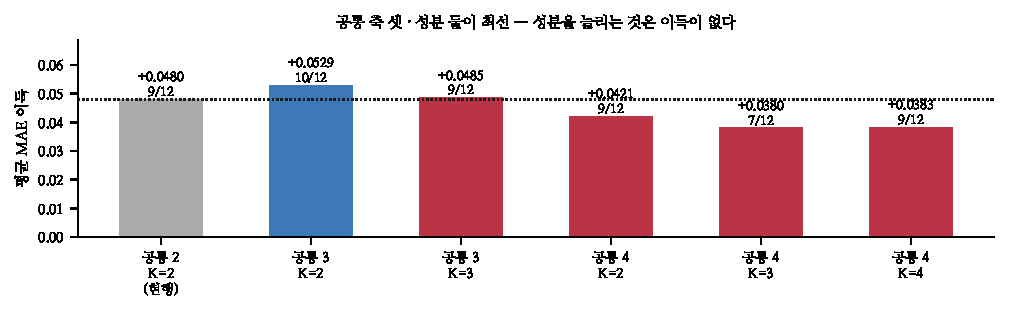
\includegraphics[width=\textwidth]{figs/cgrid.pdf}
\caption{공통 축 수와 성분 수의 격자. 점선이 현행이다.}
\end{figure}

\begin{table}[t]
\centering\tsize
\caption{결측 판정을 고친 뒤. 게임 482건이 전부 살아 있다.}
\begin{tabular}{lrr}
\toprule
설정 & 유의 & 평균 이득 \\
\midrule
공통 2 · K$=$2 (현행) & 9/12 & $+$0.0480 \\
\textbf{공통 3 · K$=$2} & \textbf{10/12} & \textbf{$+$0.0529} \\
공통 3 · K$=$3 & 9/12 & $+$0.0485 \\
공통 4 · K$=$2 & 9/12 & $+$0.0421 \\
공통 4 · K$=$3 & 7/12 & $+$0.0380 \\
공통 4 · K$=$4 & 9/12 & $+$0.0383 \\
\bottomrule
\end{tabular}
\end{table}

세 가지가 읽힌다.

\begin{itemize}[leftmargin=1.1em,itemsep=0.15em]
\item \textbf{공통 축 셋이 낫다.} 9/12 $\to$ 10/12, 이득 10\% 증가.
      팝업$\to$도서가 처음으로 유의해졌다(p$=$0.017).
\item \textbf{성분을 늘리는 것은 이득이 없다.} 공통 축이 셋이어도 K$=$3은
      K$=$2보다 나쁘다(9/12 대 10/12). 노트 36이 ``$k\le c$라서 묶여 있다''고
      본 것은 제약이 있다는 뜻이지 그 제약이 구속하고 있다는 뜻이 아니었다.
\item \textbf{입장 허들은 공통 축이 아니다.} 넷으로 늘리면 나빠진다. 가격은
      도메인마다 다른 것을 잰다는 노트 9·16의 판단이 세 번째로 확인된다.
\end{itemize}

\section{그런데 가설은 틀렸다}

공통 축을 늘려 좋아졌으니 노트 36의 가설이 맞은 것처럼 보인다. 확인하려고
여섯 설정 $\times$ 네 대상, 스물네 점에서 전이 상관을 무엇이 설명하는지 다시 쟀다.

\begin{figure}[t]
\centering
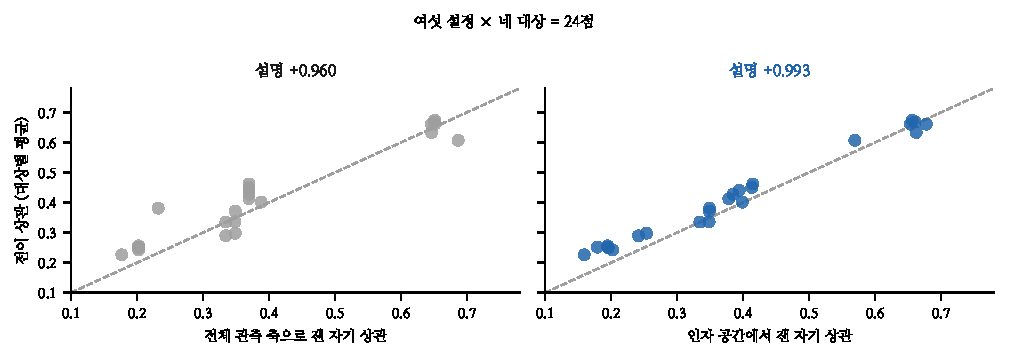
\includegraphics[width=\textwidth]{figs/where.pdf}
\caption{같은 24점을 두 가지 자기 상관에 대해 그린 것.}
\end{figure}

\begin{table}[t]
\centering\tsize
\caption{전이 상관을 무엇이 설명하나(24점).}
\begin{tabular}{lr}
\toprule
후보 & 전이 r과의 상관 \\
\midrule
전체 관측 축으로 잰 자기 상관 & $+$0.960 \\
\textbf{인자 공간에서 잰 자기 상관} & \textbf{$+$0.993} \\
\bottomrule
\end{tabular}
\end{table}

노트 36이 반례라고 내세운 사례들을 다시 본다.

\begin{table}[t]
\centering\tsize
\caption{노트 36의 ``반례''. 인자 공간에서 보면 반례가 아니다.}
\begin{tabular}{llrrr}
\toprule
설정 & 대상 & 전체 축 & 인자 공간 & 전이 \\
\midrule
현행 & 아이돌 & $+$0.651 & $+$0.656 & $+$0.673 \\
고유 확장 & 아이돌 & \textbf{$+$0.687} & \textbf{$+$0.569} & \textbf{$+$0.607} \\
\midrule
현행 & 팝업 & $+$0.370 & $+$0.385 & $+$0.427 \\
고유 확장 & 팝업 & \textbf{$+$0.232} & \textbf{$+$0.349} & \textbf{$+$0.381} \\
\bottomrule
\end{tabular}
\end{table}

아이돌은 전체 축 자기 상관이 올랐는데(0.651$\to$0.687) 인자 공간에서는
떨어졌고(0.656$\to$0.569) 전이도 그만큼 떨어졌다(0.673$\to$0.607). 팝업은 전체
축이 크게 떨어졌는데(0.370$\to$0.232) 인자 공간은 조금만 떨어졌고(0.385$\to$0.349)
전이도 조금만 떨어졌다(0.427$\to$0.381).

\textbf{둘 다 인자 공간 자기 상관을 따라간다.} 노트 36에서 반례로 보인 것은
자기 상관을 전이가 쓰지 않는 자리에서 쟀기 때문이었다.

\claimx{전이 상관은 대상 도메인이 \emph{전이가 실제로 통과하는 인자 공간}으로
자기 라벨을 설명하는 정도와 같다(24점에서 $+$0.993). 상한은 하나이고 노트 36의
두 상한 가설은 기각한다.}{인자 공간 자기 상관이 같은데 전이가 크게 다른 두
설정이 나오면 이 하나의 상한으로도 부족한 것이다.}

\section{그러면 무엇이 바뀌나}

\begin{figure}[t]
\centering
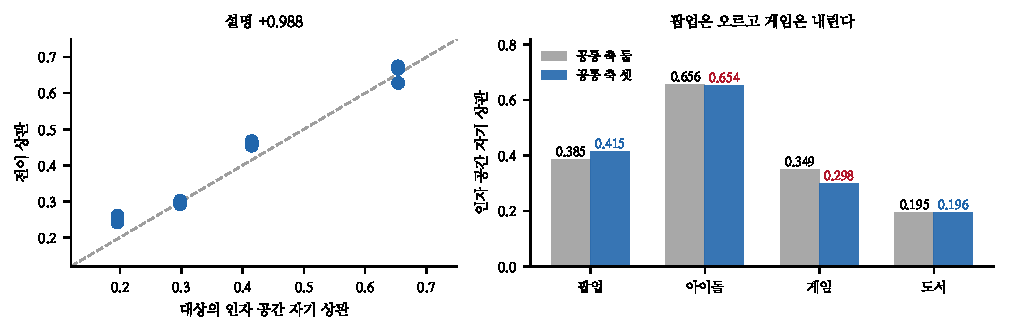
\includegraphics[width=\textwidth]{figs/now.pdf}
\caption{왼쪽 --- 채택 후 열두 셀. 오른쪽 --- 도메인별 인자 공간 자기 상관 변화.}
\end{figure}

공통 축을 셋으로 늘린 것이 왜 좋았는지도 이제 설명된다. 그것이 ``정렬 전달력''을
올려서가 아니라 \textbf{팝업의 인자 공간 자기 상관을 0.385에서 0.415로 올렸기}
때문이다. 게임은 0.349에서 0.298로 내려갔고 게임을 대상으로 한 세 셀이 전부
나빠졌다 --- 등식대로다. 순 효과가 이득이라 채택했다.

\begin{quote}\fontsize{9.5}{11.5}\selectfont
실무 규칙이 다시 쓰인다. 노트 36은 ``고유 축이 아니라 공통 축을 늘려라''라고
했다. 정확하게는 --- \textbf{축을 늘리는 것이 목적이 아니라, 대상 도메인의 인자
공간 자기 상관을 올리는 것이 목적이다.} 어떤 축이 그것을 올릴지는 검정으로만
알 수 있고, 공통 축이든 고유 축이든 상관없다.
\end{quote}

\paragraph{측정 가능한 목표가 생겼다}
인자 공간 자기 상관은 \emph{대상 도메인 안에서만} 계산된다. 전이를 돌릴 필요도,
다른 도메인이 있을 필요도 없다. 즉 배선 후보를 평가할 때 열두 셀을 다시 돌리는
대신 이 값 하나만 보면 된다. 노트 32가 요구한 ``라벨 없는 대리 추정''은 아니지만
--- 여전히 대상 라벨이 필요하다 --- 훨씬 싼 판정 기준이다.

\section{한계}

\begin{itemize}[leftmargin=1.1em,itemsep=0.15em]
\item 인자 공간 자기 상관은 그 도메인의 라벨을 쓴다. 노트 32의 문제(라벨 없이
      전이 성공을 예측하기)는 그대로 남아 있다.
\item 24점 중 여섯 설정이 서로 독립이 아니다. 같은 데이터를 다르게 배선한 것이라
      $+$0.993은 낙관적일 수 있다.
\item 게임 인자 공간 자기 상관이 0.349에서 0.298로 떨어진 것을 감수하고 채택했다.
      게임을 대상으로 쓸 일이 많다면 잘못된 선택이다.
\item 비율 평균이 1.100으로 1을 넘는다. 전이가 상한을 넘는 것은 여전히 이상하며
      교차검증의 보수성으로만 설명하고 있다.
\item 성분 수를 늘리는 것이 왜 이득이 없는지 모른다. 인자 공간을 넓혀도 자기
      상관이 안 오른다는 뜻인데 확인하지 않았다.
\end{itemize}

\section{다음}

\begin{enumerate}[leftmargin=1.3em,itemsep=0.15em]
\item 인자 공간 자기 상관을 목표로 두고 네 도메인의 배선을 다시 훑는다 ---
      이제 판정이 싸므로 후보를 많이 시도할 수 있다.
\item 게임의 인자 공간 자기 상관 하락을 되돌릴 배선이 있는지.
\item 결측 판정을 값 배열에서 분리하는 표현 --- 같은 실수를 세 번 하지 않도록.
\item 비율이 1을 넘는 원인 --- 교차검증 폴드 수를 바꿔 확인한다.
\end{enumerate}

\vspace{0.6em}
\hrule height 0.3pt
\vspace{0.5em}
{\footnotesize
\textbf{참고문헌}\\[0.3em]
Schönemann, P. H. (1966). A generalized solution of the orthogonal Procrustes
problem. \emph{Psychometrika}, 31(1), 1--10.\\[0.15em]
Ben-David, S. et al. (2010). A theory of learning from different domains.
\emph{Machine Learning}, 79(1--2), 151--175.\\[0.15em]
Rubin, D. B. (1976). Inference and missing data. \emph{Biometrika}, 63(3), 581--592.\\[0.15em]
Kaufman, S., Rosset, S., Perlich, C. (2012). Leakage in data mining.
\emph{ACM TKDD}, 6(4), 1--21.\\[0.15em]
Meredith, W. (1993). Measurement invariance, factor analysis and factorial
invariance. \emph{Psychometrika}, 58(4), 525--543.
}

\end{document}
